\cleardoublepage

{
    \sectionnonum{附录}

    \appendixsubsecmajornumbering

    \subsection{本论文中使用的代码}

    \begin{lstlisting}[%
        language={C++},
        caption={射线法},
        label={code:ray}
    ]
    int countIntersections(Point point, Point p1, Point p2) {
        // 计算交点个数
        if ((p1.y <= point.y && p2.y > point.y) || 
        (p1.y > point.y && p2.y <= point.y)) {
            double slope = (p2.x - p1.x) / (p2.y - p1.y);
            double intersectX = p1.x + (point.y - p1.y) * slope;
            if (point.x < intersectX) {
                return 1;
            }
        }
        return 0;
    }
    bool isPointInTriangle_Ray(Point p,Triangle t){
        int count;
        // 统计与三角形边的交点个数
        count = countIntersections(p, t.p1, t.p2) +
                    countIntersections(p, t.p2, t.p3) +
                    countIntersections(p, t.p3, t.p1);
        // 判断点是否在三角形内部
        return count % 2 == 1;
    }
    \end{lstlisting}
    \begin{lstlisting}[%
        language={C++},
        caption={面积法},
        label={code:square}
    ]
    
    // 计算三角形的面积
    double triangleArea(Triangle triangle) {
        return abs(0.5 * crossProduct(triangle.p1, 
        triangle.p2, triangle.p3));
    }
    
    // 判断点是否在三角形内部(面积法)
    bool isPointInTriangle_Area(Point point, Triangle triangle) {
        double totalArea,area1,area2,area3;
        // 计算三角形的总面积
        totalArea = triangleArea(triangle);
        // 计算点到各个顶点的子三角形的面积之和
        area1 = triangleArea({point, triangle.p1, triangle.p2});
        area2 = triangleArea({point, triangle.p2, triangle.p3});
        area3 = triangleArea({point, triangle.p1, triangle.p3});
    
        // 判断点是否在三角形内部
        return totalArea == (area1 + area2 + area3);
    }
    
    
    \end{lstlisting}

    
    \begin{lstlisting}[%
        language={C++},
        caption={边界方程法},
        label={code:edge function}
    ]
    
    bool isPointInTriangle_EdgeFunction(Point p,Triangle t)
    {
        double cp1,cp2,cp3;
    
        cp1 = crossProduct(t.p1,t.p2,p);
        cp2 = crossProduct(t.p2,t.p3,p);
        cp3 = crossProduct(t.p3,t.p1,p);
    
        if((cp1<0 && cp2<0 && cp3 < 0)||
        (cp1 > 0 && cp2 > 0 && cp3 > 0))
        {
            return true;
        }
        else return false;
    }
    \end{lstlisting}


    \begin{lstlisting}[%
        language={C++},
        caption={三角形测试算法性能测试},
        label={code:test},
    ]
    #include"StructDef.h"
    #include"PointInTriangle.h"
    int main() {
        // 随机生成点和三角形
        srand(time(nullptr));
        Point point{static_cast<double>(rand()) / RAND_MAX, static_cast<double>(rand()) / RAND_MAX};
        Triangle triangle = {
            {static_cast<double>(rand()) / RAND_MAX, static_cast<double>(rand()) / RAND_MAX},
            {static_cast<double>(rand()) / RAND_MAX, static_cast<double>(rand()) / RAND_MAX},
            {static_cast<double>(rand()) / RAND_MAX, static_cast<double>(rand()) / RAND_MAX}
        };
        int count = 1E7;
        int unit = 1E3;
        bool resultArea,resultRay,resultBoundary;
        // 测试面积法性能
        clock_t start = clock();
        for(int i=0;i<count;++i)
            resultArea = isPointInTriangle_Area(point, triangle);
        clock_t end = clock();
        double elapsedTimeArea = (double(end - start) / CLOCKS_PER_SEC)/(count/unit);
    
        // 测试射线法性能
        start = clock();
        for(int i=0;i<count;++i)
            resultRay = isPointInTriangle_Ray(point, triangle);
        end = clock();
        double elapsedTimeRay = (double(end - start) / CLOCKS_PER_SEC)/(count/unit);
    
        // 测试边界方程法性能
        start = clock();
        for(int i=0;i<count;++i)
            resultBoundary = isPointInTriangle_EdgeFunction(point, triangle);
        end = clock();
        double elapsedTimeBoundary = (double(end - start) / CLOCKS_PER_SEC)/(count/unit);
    
        // 输出结果
        std::cout << "test" <<std::endl;
        std::cout << "Point: (" << point.x << ", " << point.y << ")" << std::endl;
        std::cout << "Triangle: (" << triangle.p1.x << ", " << triangle.p1.y << "), "
                  << "(" << triangle.p2.x << ", " << triangle.p2.y << "), "
                  << "(" << triangle.p3.x << ", " << triangle.p3.y << ")" << std::endl;
        std::cout << "Is inside triangle (Area method): " << std::boolalpha << resultArea << ", Time: " << elapsedTimeArea << " ms" << std::endl;
        std::cout << "Is inside triangle (Ray method): " << std::boolalpha << resultRay << ", Time: " << elapsedTimeRay << " ms" << std::endl;
        std::cout << "Is inside triangle (Boundary method): " << std::boolalpha << resultBoundary << ", Time: " << elapsedTimeBoundary << " ms" << std::endl;
    
        return 0;
    }
    
    \end{lstlisting}
    


    \begin{lstlisting}[%
        language={C++},
        caption={三种测试算法的并行化实现},
        label={code:test parallel version}
    ]
    #include"PointInTriangle.h"
    // 边界方程法
    bool isPointInTriangle_EdgeFunction(Point p,Triangle t)
    {
        double cp1,cp2,cp3;
        std::vector<std::pair<double,std::vector<Point>>> list{
            std::pair<double,std::vector<Point>>(0,std::vector<Point>{t.p1,t.p2,p}),
            std::pair<double,std::vector<Point>>(0,std::vector<Point>{t.p2,t.p3,p}),
            std::pair<double,std::vector<Point>>(0,std::vector<Point>{t.p3,t.p1,p})
        };
        std::for_each(std::execution::par,list.begin(),list.end(),[](std::pair<double,std::vector<Point>>& it){
            it.first = crossProduct(it.second[0],it.second[1],it.second[2]);
        });
        cp1 = list[0].first;
        cp2 = list[1].first;
        cp3 = list[2].first;

        if((cp1<0 && cp2<0 && cp3 < 0)||(cp1>0&&cp2>0&&cp3>0))
        {
            return true;
        }
        else return false;
    }
    // 计算三角形的面积
    double triangleArea(Triangle triangle) {
        return abs(0.5 * crossProduct(triangle.p1, triangle.p2, triangle.p3));
    }
    
    // 判断点是否在三角形内部(面积法)
    bool isPointInTriangle_Area(Point point, Triangle triangle) {
        double totalArea,area1,area2,area3;
        std::vector<std::pair<double,std::vector<Point>>> list{
            std::pair<double,std::vector<Point>>(0,std::vector<Point>{triangle.p3,triangle.p1,triangle.p2}),
            std::pair<double,std::vector<Point>>(0,std::vector<Point>{point,triangle.p1,triangle.p2}),
            std::pair<double,std::vector<Point>>(0,std::vector<Point>{point,triangle.p2,triangle.p3}),
            std::pair<double,std::vector<Point>>(0,std::vector<Point>{point,triangle.p1,triangle.p3})
        };
        std::for_each(std::execution::par,list.begin(),list.end(),[](std::pair<double,std::vector<Point>>& it){
            it.first = triangleArea({it.second[0],it.second[1],it.second[2]});
        });
        totalArea = list[0].first;
        area1 = list[1].first;
        area2 = list[2].first;
        area3 = list[3].first;

        // 判断点是否在三角形内部
        return totalArea == (area1 + area2 + area3);
    }
    
    // 定义射线与边的交点计数函数
    int countIntersections(Point point, Point p1, Point p2) {
        // 计算交点个数
        if ((p1.y <= point.y && p2.y > point.y) || (p1.y > point.y && p2.y <= point.y)) {
            double slope = (p2.x - p1.x) / (p2.y - p1.y);
            double intersectX = p1.x + (point.y - p1.y) * slope;
            if (point.x < intersectX) {
                return 1;
            }
        }
        return 0;
    }
    
    // 判断点是否在三角形内部(射线法)
    
    bool isPointInTriangle_Ray(Point p,Triangle t){
        int count;
        std::vector<std::pair<int,std::vector<Point>>> list{
            std::pair<int,std::vector<Point>>(0,std::vector<Point>{p,t.p1,t.p2}),
            std::pair<int,std::vector<Point>>(0,std::vector<Point>{p,t.p2,t.p3}),
            std::pair<int,std::vector<Point>>(0,std::vector<Point>{p,t.p3,t.p1})
        };
        std::for_each(std::execution::par,list.begin(),list.end(),[](std::pair<int,std::vector<Point>>& it){
            it.first = countIntersections(it.second[0],it.second[1],it.second[2]);
        });
        count = list[0].first+list[1].first+list[2].first;

        // 判断点是否在三角形内部
        return count % 2 == 1;
    }

    \end{lstlisting}

    \subsection{流程图}
    \begin{figure}[H]
        \centering
        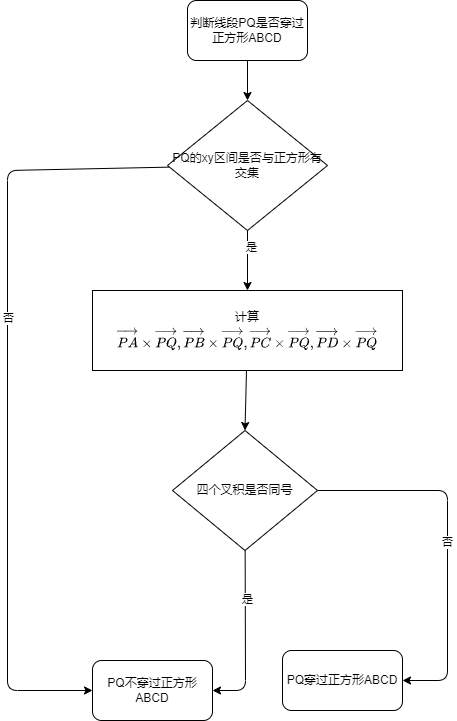
\includegraphics[width=.9\textwidth]{figure/linethroughrectangle.png}
        \caption{线段穿过tile的判断流程}
        \label{fig:line through tile flow chart}
    \end{figure}
    \begin{figure}[H]
        \centering
        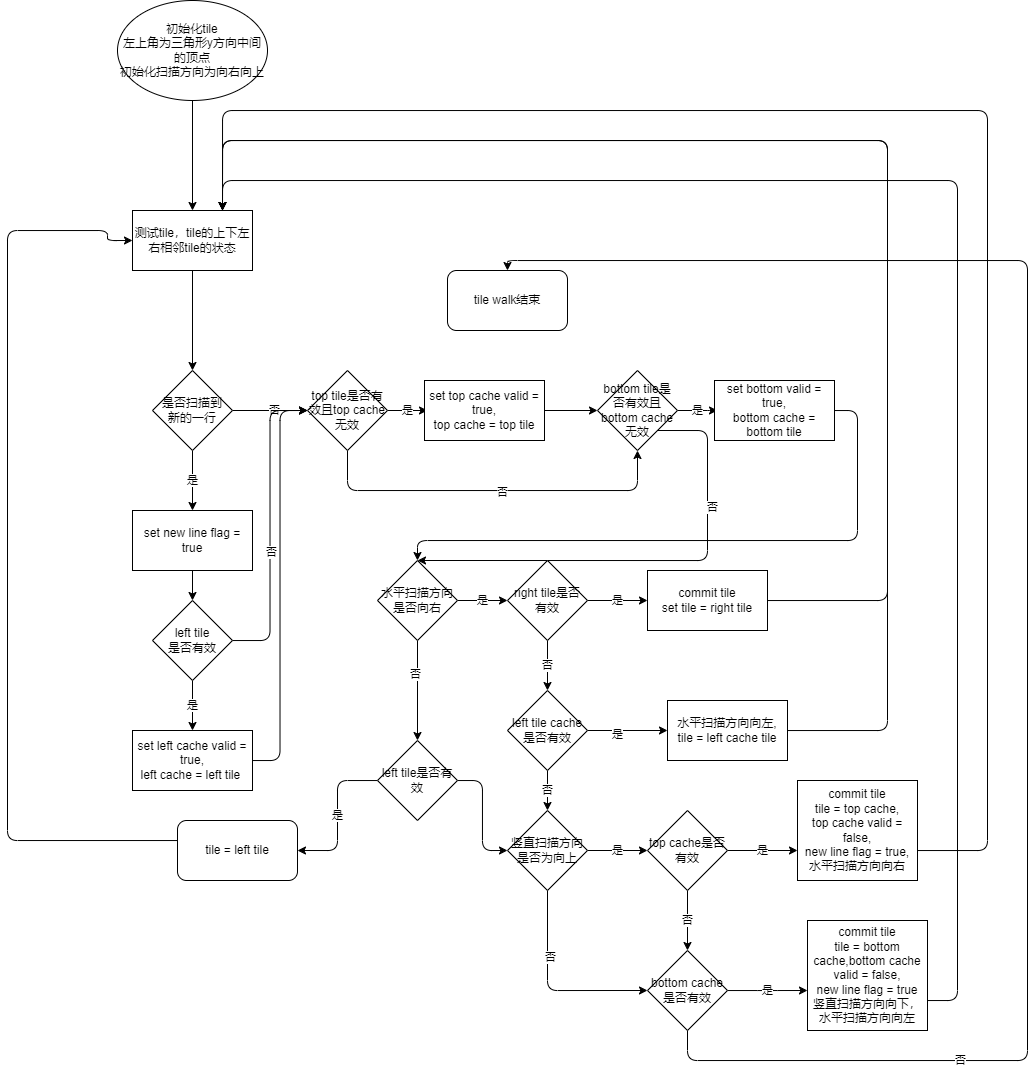
\includegraphics[width=.9\linewidth]{figure/tilewalkflow.png}
        \caption{\label{fig:tile scan flow chart}tile扫描流程}
    \end{figure}
    \begin{figure}[H]
        \centering
        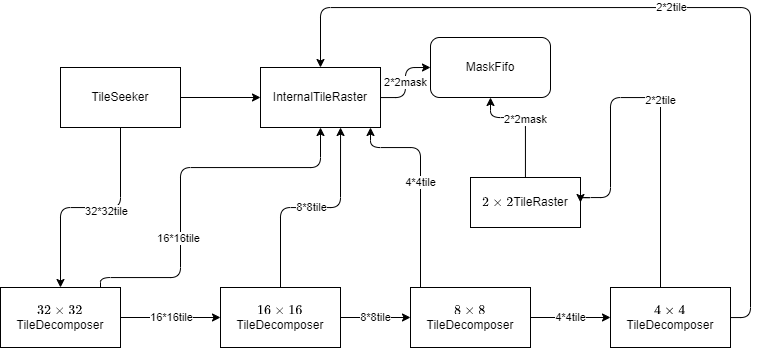
\includegraphics[width=.9\linewidth]{figure/pipeline.png}
        \caption{\label{fig:alogrithm pipeline}测试算法流水线}
    \end{figure}
    

    \begin{figure}[H]
        \centering
        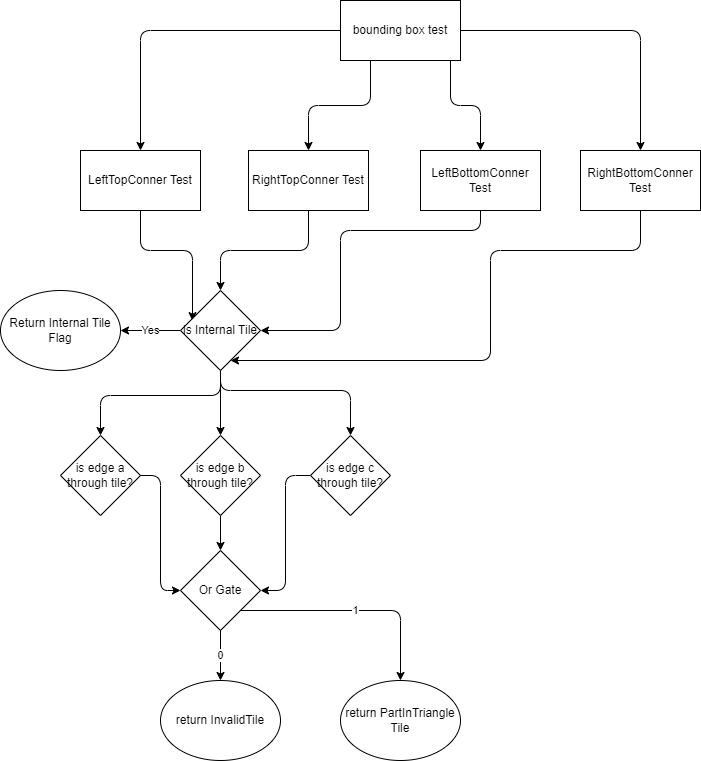
\includegraphics[width=.9\textwidth]{figure/tilechekflow.png}
        \caption{\label{fig:tile check topo flow}tile类型判断的过程}
    \end{figure}


    \subsection{100个随机三角形数据集}
    \begin{lstlisting}[%
        language={C++},
        caption={100个随机三角形},
        label={data:100 random triangles}
    ]
    228 469 286 364 551 1
    204 223 196 21 185 473
    200 168 59 0 395 420
    703 412 706 197 663 329
    671 369 713 235 219 535
    502 431 474 375 379 252
    220 122 137 11 360 141
    753 600 758 574 363 326
    501 272 740 223 285 94
    693 541 666 371 161 441
    800 149 726 40 479 459
    526 99 641 47 771 547
    663 384 719 242 555 129
    151 376 44 257 307 369
    504 486 741 469 577 103
    113 481 360 369 470 498
    581 408 644 293 436 184
    376 226 490 202 53 256
    286 464 201 326 656 182
    312 600 326 456 234 155
    639 436 710 313 463 557
    655 189 738 104 266 482
    175 240 216 143 563 411
    534 126 553 0 170 204
    542 252 759 99 637 319
    356 478 466 304 304 167
    365 134 428 22 577 525
    363 25 566 14 417 548
    440 600 247 409 273 487
    713 329 786 187 42 148
    574 237 800 165 778 80
    646 299 666 104 700 305
    0 251 121 31 618 78
    132 192 135 153 139 6
    347 268 369 11 600 112
    451 215 516 139 56 445
    369 561 460 516 282 560
    106 344 347 338 181 555
    788 398 665 223 543 376
    356 219 420 127 226 415
    253 102 404 10 283 232
    784 324 800 139 796 391
    672 362 663 256 496 156
    467 600 573 448 391 482
    767 600 770 403 142 87
    220 600 287 483 537 235
    13 465 171 324 143 504
    721 470 800 462 391 19
    633 396 651 171 607 346
    800 600 800 522 578 522
    60 254 154 142 424 464
    800 600 744 481 275 105
    376 600 446 480 148 552
    564 271 699 241 678 421
    525 441 728 387 621 576
    460 352 637 272 23 269
    494 161 733 158 94 554
    0 69 173 52 253 496
    76 438 107 347 489 197
    605 174 766 79 658 479
    544 226 659 0 129 360
    792 567 708 511 376 470
    83 600 156 534 257 306
    800 387 800 269 645 330
    217 201 364 0 476 94
    596 444 770 392 495 476
    458 442 401 234 113 290
    637 150 576 39 753 469
    153 113 229 35 746 248
    50 353 163 346 391 33
    362 269 504 251 580 276
    170 450 370 375 713 107
    788 365 681 213 525 250
    768 369 673 250 617 389
    751 373 551 274 294 319
    605 483 799 376 465 288
    0 600 211 574 611 94
    334 338 267 120 668 177
    267 176 263 116 26 155
    0 549 75 515 665 389
    236 483 34 301 139 202
    278 275 435 73 74 487
    173 579 324 572 405 147
    487 251 512 87 624 286
    362 193 628 175 423 8
    622 527 708 387 352 451
    242 456 138 241 619 153
    255 512 390 416 619 31
    635 391 800 360 127 84
    0 97 71 85 253 92
    172 163 282 110 249 189
    624 468 782 408 360 508
    185 511 348 499 309 183
    497 213 764 82 372 106
    68 140 61 0 524 39
    296 600 262 460 516 421
    343 311 509 96 574 81
    448 472 399 387 3 459
    236 541 218 407 574 298
    292 600 435 547 301 393
    \end{lstlisting}
    % End of appendix
    \removeappendixsubsecmajornumbering
}

\subsection{项目总结}

本研究成功设计并实现了一种适合国产 GPU 架构的高效 Point-in-Triangle 并行测试算法,通过性能测试验证了测试系统在处理速度、资源消耗方面的均衡性,测试系统在吞吐量较高使得下游模块能够饱和工作的同时,规划减少了资源的消耗,并且具有高度的可延展性,适应不同的时钟频率,能够支持不同数量的并行运算单元和不同的流水线深度。



